% -*- mode: latex; -*- mustache tags:  
\documentclass[10pt,twoside,english]{_support/latex/sbabook/sbabook}
\let\wholebook=\relax

\usepackage{import}
\subimport{_support/latex/}{common.tex}

%=================================================================
% Debug packages for page layout and overfull lines
% Remove the showtrims document option before printing
\ifshowtrims
  \usepackage{showframe}
  \usepackage[color=magenta,width=5mm]{_support/latex/overcolored}
\fi


% =================================================================
\title{Pharo Graphics}
\author{The Pillar team}
\series{Square Bracket tutorials}

\hypersetup{
  pdftitle = {Pharo Graphics},
  pdfauthor = {The Pillar team},
  pdfkeywords = {graphics, canvas}
}


% =================================================================
\begin{document}

% Title page and colophon on verso
\maketitle
\pagestyle{titlingpage}
\thispagestyle{titlingpage} % \pagestyle does not work on the first one…

\cleartoverso
{\small

  Copyright 2017 by The Pillar team.

  The contents of this book are protected under the Creative Commons
  Attribution-ShareAlike 3.0 Unported license.

  You are \textbf{free}:
  \begin{itemize}
  \item to \textbf{Share}: to copy, distribute and transmit the work,
  \item to \textbf{Remix}: to adapt the work,
  \end{itemize}

  Under the following conditions:
  \begin{description}
  \item[Attribution.] You must attribute the work in the manner specified by the
    author or licensor (but not in any way that suggests that they endorse you
    or your use of the work).
  \item[Share Alike.] If you alter, transform, or build upon this work, you may
    distribute the resulting work only under the same, similar or a compatible
    license.
  \end{description}

  For any reuse or distribution, you must make clear to others the
  license terms of this work. The best way to do this is with a link to
  this web page: \\
  \url{http://creativecommons.org/licenses/by-sa/3.0/}

  Any of the above conditions can be waived if you get permission from
  the copyright holder. Nothing in this license impairs or restricts the
  author's moral rights.

  \begin{center}
    
\includegraphics[width=0.2\textwidth]{_support/latex/sbabook/CreativeCommons-BY-SA.pdf}
  \end{center}

  Your fair dealing and other rights are in no way affected by the
  above. This is a human-readable summary of the Legal Code (the full
  license): \\
  \url{http://creativecommons.org/licenses/by-sa/3.0/legalcode}

  \vfill

  % Publication info would go here (publisher, ISBN, cover design…)
  Layout and typography based on the \textcode{sbabook} \LaTeX{} class by Damien
  Pollet.
}


\frontmatter
\pagestyle{plain}

\tableofcontents*
\clearpage\listoffigures

\mainmatter


\chapter{Vector graphics in Athens}
There are two different computer graphics: vector and raster graphics.
Raster graphics represent images as a collection of pixels. Vector graphics
is the use of geometric primitives such as points, lines, curves, or polygons
to represent images. These primitives are created using mathematical equations.

Both types of computer graphics have advantages and disadvantages.
The advantages of vector graphics over raster are:

\begin{itemize}
    \item smaller size,
    \item ability to zoom indefinitely,
    \item moving, scaling, filling, and rotating do not degrade the quality of an image.
\end{itemize}

Ultimately, pictures on a computer are displayed on a screen with a specific
display dimension. However, while raster graphics doesn't scale very well when
the resolution differs too much from the picture resolution, vector graphics
are rasterized to fit the display they will appear on. Rasterization is the
technique of taking an image described in a vector graphics format and
transforming it into a set of pixels for output on a screen.

Morphic is the way to do graphics with Pharo.
However, most existing canvases are pixel based, and not vector based.
This can be an issue with current IT ecosystems, where the resolution can differ from machine to machine (desktop, tablet, phones, etc...)

Enter Athens, a vector-based graphic API. Under the scene, it can either use
balloon Canvas, or the Cairo graphic library for the rasterization phase.

\section{Example}
By the end of this chapter, you will be able to understand the example below:
SD: problem with parentheses.
\begin{displaycode}{smalltalk}
| surface |
surface := AthensCairoSurface   extent: 400@400.

surface drawDuring: [ :canvas | 

	| paint font |
	paint := (PolymorphSystemSettings pharoLogoForm) asAthensPaintOn: canvas.
 
	canvas setPaint: (
		 (LinearGradientPaint from: 0@0  to: 400@400) 
			 colorRamp: {  
			  0 -> (Color red alpha: 0.8).
			  0.166 -> (Color orange alpha: 0.8).
			  0.332 -> (Color yellow alpha: 0.8).
			  0.5 -> (Color green alpha: 0.8).
			  0.664 -> (Color blue alpha: 0.8).
			  0.83 -> (Color magenta alpha: 0.8).
			  1 -> (Color purple alpha: 0.8). 
		 }).

canvas drawShape: (0@0 extent: 400@400). 
paint maskOn: canvas.
 
font := LogicalFont familyName: 'Source Sans Pro' pointSize: 30.
canvas setFont: font.
canvas setPaint:(  (LinearGradientPaint from: 0@0  to: 100@150)
 colorRamp: {  
  0 -> (Color white alpha: 0.9).
  1 -> (Color black alpha: 0.9).}).
canvas pathTransform translateX: 20 Y: 180 + (font getPreciseAscent); scaleBy: 1.1; rotateByDegrees: 25.

canvas drawString: 'Hello Athens in Pharo'

"canvas draw."
].

surface asForm
\end{displaycode}

\section{Athens details}
\textcode{AthensSurface} and its subclass \textcode{AthensCairoSurface} will initialize a new surface.
The surface represents the area in pixels where your drawing will be rendered. You
never draw directly on the surface. Instead, you specify what you want to display
on the canvas, and Athens will render it on the area specified by the surface.

The class \textcode{AthensCanvas} is the central object used to perform drawing on an \textcode{AthensSurface}
A canvas is not directly instantiated but used through a call like\textcode{surface drawDuring: {[}:canvas \textbar{} .... {]}}

The Athens drawing model relies on a three-layer model. Any drawing process
takes place in three steps:

\begin{itemize}
    \item First, a painting must be defined, which may be a color, a color gradient, or a bitmap.
    \item Then a \textcode{path} is created, which includes one or more vector primitives, i.e., lines, TrueType fonts, B\'{e}zier curves, etc... This path will define the shape that is then rendered.
    \item Finally, the result is drawn to the Athens surface, which is provided by the back-end for the output.
\end{itemize}

\subsection{Paint}
Paint can be:

\begin{itemize}
    \item a single color, defined with the message \textcode{color:}
    \item A radial gradient paint, defined through object \textcode{RadialGradientPaint}
    \item a linear gradient paint, defined through object \textcode{LinearGradientPaint}
    \item a bitmap you can get by sending \textit{asAthensPaintOn:} to a \textcode{Form}.
\end{itemize}

The way the paint is applied in the canvas is specified as \textit{Fill} or \textit{Stroke} that we will see in detail:

\begin{itemize}
    \item \textcode{setPaint:} message will fill the Paint in the area defined by the path.
    \item \textcode{setStrokePaint:} message will set the paint as a virtual pen along the path.
\end{itemize}

Let's see some examples to better understand how it works.

\subsection{Stroke paint (a pen that goes around the path)}
The stroke operation takes a virtual pen along the path. It allows the source to transfer through the mask in a thin (or thick) line around the path
\begin{displaycode}{smalltalk}
|surface|
surface := AthensCairoSurface extent: 200@200.

surface drawDuring: [ :canvas | 
        surface clear: Color white.
        canvas setStrokePaint:  Color red.
        canvas drawShape: (20@20 extent: 160@160). 
].

surface asForm
\end{displaycode}

The paint can be customized like
\begin{displaycode}{smalltalk}
|surface|
surface := AthensCairoSurface extent: 200@200.

surface drawDuring: [ :canvas | 
        surface clear: Color white.
        canvas setStrokePaint:  Color red.
        canvas paint dashes: #( "fill"5   "gap" 15) offset: 5.
        canvas paint capSquare.
        canvas paint width: 10.
        canvas drawShape: (20@20 extent: 160@160). 
].

surface asForm
\end{displaycode}

\subsection{Fill paint (a paint that fill the area defined by the path)}
A gradient will let you create a gradient of color, either linear or radial.

The color ramp is a collection of associations with keys - floating point values
between 0 and 1 and values with Colors, for example:
\begin{displaycode}{smalltalk}
{0 -> Color blue . 0.5 -> Color white. 1 -> Color red}.
\end{displaycode}

Full example with all paints:

Paint bitmap needs to be moved to the place you want to have them drawn. Otherwise, they will stay in the top left corner of the surface area. The message \textcode{loadIdentity} is necessary for the next paint as the previous \textcode{paintTransform} will continue to apply to the new paint definition.

We can use the same paint definition with stroke paint move. However, in this situation, the paint will only appear in the thickness of the stroke line.
\begin{displaycode}{smalltalk}
|surface|
surface := AthensCairoSurface extent: 200@200.

surface drawDuring: [ :canvas |
surface clear: (Color purple alpha: 0.3).
"linear gradient fill"
    canvas setPaint:  ((LinearGradientPaint from: 0@0  to: 100@100) colorRamp: {  0 -> Color white. 1 -> Color black }).
    canvas drawShape: (0@0 extent: 100@100).

"plain color fill"
    canvas setPaint:  (Color yellow alpha: 0.9).
    canvas drawShape: (100@0 extent: 200@100).

"Bitmap fill"
    canvas setPaint: (PolymorphSystemSettings pharoLogoForm asAthensPaintOn: canvas ).
    canvas paintTransform translateX: 0 Y: 135.
    canvas paintTransform scaleBy: 0.25.
    canvas drawShape: (0@100 extent: 100@200).

"Radial gradient fill"
    canvas paintTransform loadIdentity.
    canvas setPaint: ((RadialGradientPaint new) colorRamp: { 0 -> Color white. 1 -> Color black }; center: 150@150; radius: 50; focalPoint: 180@180).
    canvas drawShape: (100@100 extent: 200@200).

 ].
surface asForm 
\end{displaycode}

Start and stop points are references to the current shape being drawn.
Example:
Create a vertical gradient
\begin{displaycode}{smalltalk}
canvas
    setPaint:
        (canvas surface
            createLinearGradient:
                {(0 -> Color blue).
                (0.5 -> Color white).
                (1 -> Color red)}
            start: 0@200
            stop: 0@400). 
    canvas drawShape: (0@200 extent: 300@400).
\end{displaycode}

Create a horizontal gradient:
\begin{displaycode}{smalltalk}
canvas
    setPaint:
        (canvas surface
            createLinearGradient:
                {(0 -> Color blue).
                (0.5 -> Color white).
                (1 -> Color red)}
            start: 0@200
            stop: 300@200). 
    canvas drawShape: (0@200 extent: 300@400).
\end{displaycode}

Create a diagonal gradient:
\begin{displaycode}{smalltalk}
canvas
    setPaint:
        (canvas surface
            createLinearGradient:
                {(0 -> Color blue).
                (0.5 -> Color white).
                (1 -> Color red)}
            start: 0@200
            stop: 300@400). 
    canvas drawShape: (0@200 extent: 300@400).
\end{displaycode}

\section{Path}
Athens always has an active path.

Use \textcode{AthensPathBuilder} or \textcode{AthensSimplePathBuilder} to build a path
They will assemble segments for you

The method \textcode{createPath:} exists in all important Athens class: \textcode{AthensCanvas},\textcode{AthensSurface}, and  \textcode{AthensPathBuilder}.
The message \textcode{createPath: aPath}

Using it returns a new path:
\begin{displaycode}{smalltalk}
surface createPath: [:builder |
  builder
   absolute;
   moveTo: 100@100;
   lineTo: 100@300;
   lineTo: 300@300;
   lineTo: 300@100;
   close ].
\end{displaycode}

Here are some helper messages in \textcode{AthensSimplePathBuilder}:

\begin{itemize}
    \item \textcode{pathStart}
    \item \textcode{pathBounds} gives the limit of the bounds associated with the path
\end{itemize}

If you want to build a path using only a straight line, you can use the class \textcode{AthensPolygon}.

\begin{fullwidthtabular}{lll}
\toprule
path builder Messages & Object Segment & comment \\
\sout{}\sout{}\sout{}\sout{}\sout{}\textasciitilde{}- & \sout{}\sout{}\sout{}\sout{}\textasciitilde{}- & \sout{}\sout{}\sout{}\sout{}\sout{}\sout{}\sout{} \\
ccwArcTo: angle: & AthensCCWArcSegment & counter clock wise segment \\
cwArcTo:angle: & AthensCWArcSegment & clock wise segment \\
lineTo: & AthensLineSegment & straight line \\
moveTo: & AthensMoveSegment & start a new contour \\
curveVia: to: & AthensQuadSegment & quadric bezier curve \\
curveVia: and: to: & AthensCubicSegment & Cubic bezier curve \\
reflectedCurveVia: to: & AthensCubicSegment & Reflected cubic bezier curve \\
string: font: &  & specific to cairo \\
close & AthensCloseSegment & close the current contour \\
\bottomrule
\end{fullwidthtabular}

\section{Coordinate class: \textbf{Absolute} or \textbf{Relative}}
\subsection{Absolute: absolute coordinate from surface coordinate}
This will draw a square in a surface whose extent is 400@400 using an absolute move.
\begin{displaycode}{smalltalk}
builder absolute;
   moveTo: 100@100;
   lineTo: 100@300;
   lineTo: 300@300;
   lineTo: 300@100;
   close
\end{displaycode}

relative: each new move is relative to the previous one.
This will draw a square in a surface whose extent is 400@400 using relative move.
\begin{displaycode}{smalltalk}
 builder relative ;
  moveTo: 100@100;
  lineTo: 200@0;
  lineTo: 0@200;
  lineTo: -200@0;
  close
\end{displaycode}

\subsection{moving}
\begin{itemize}
    \item moveTo: -\textgreater{} move path to a specific point to \textit{initiate} drawing.
\end{itemize}

\subsection{straight line}
\begin{itemize}
    \item lineTo: line path from previous point to target point.
\end{itemize}

\subsection{arcs}
\begin{itemize}
    \item \textcode{ccwArcTo: endPt angle: rot}. Add a counter-clockwise arc segment, starting from current path endpoint and ending at andPt. Angle should be specified in radians.
    \item \textcode{cwArcTo: endPt angle: rot}. Add a clockwise arc segment, starting from current path endpoint and ending at andPt. Angle should be specified in radians.
\end{itemize}

\textcode{cwArcTo:angle:} and \textcode{ccwArcTo: angle:} will draw circular arc, connecting previous segment endpoint and current endpoint of given angle, passing in
clockwise or counter clockwise direction. The angle must be specified in Radian.

Please remember that the circumference of a circle is equal to 2 Pi  R.
If R = 1, half of the circumference is equal to PI, which is the value of half a circle.

\subsection{curves}
\begin{itemize}
    \item curveVia: cp1 and: cp2 to: aPoint. Add a cubic bezier curve starting from the current path endpoint, using control points cp1, cp2 and ending at aPoint.
    \item curveVia: cp1 to: aPoint. Add a quadric bezier curve, starting from the current path endpoint, using control point cp1, and ending at aPoint.
    \item reflectedCurveVia: cp2 to: aPoint. Add a reflected cubic bezier curve, starting from the current path endpoint and ending at aPoint. The first control point is calculated as a reflection from the current point, if the last command was also a cubic bezier curve. Otherwise, the first control point is the current point. The second control point is cp2.
\end{itemize}

\subsection{curveVia: to: and \textbar{}curveVia: and: to}
This call is related to the bezier curve. A B\'{e}zier curve consists of two or more
control points, which define the size and shape of the line. The first and
last points mark the beginning and end of the path, while the intermediate
points define the path's curvature.

More detail on Bezier curve on available at: \href{https://pomax.github.io/bezierinfo}{https://pomax.github.io/bezierinfo}

\subsection{Close the path}
\begin{itemize}
    \item close. Close the path contour, between the initial point, and the last reached point.
\end{itemize}

Here is a full example with all family of paths.
\begin{displaycode}{smalltalk}
| surface |
surface := AthensCairoSurface extent: 100@100.

surface drawDuring: [ :canvas |
 surface clear: Color white.
   canvas setStrokePaint: Color red.
 canvas paint width: 5.
   canvas drawShape: (
  canvas createPath: [ :builder | 
       builder
        absolute;
      moveTo: 25@25;
      lineTo: 50@37.5;
   relative;
      lineTo: 25@(-12.5);
   absolute;
   cwArcTo: 75 @ 75 angle: 90 degreesToRadians;
   curveVia: 50@60 and: 50@90 to: 25@75;
      close
  ]
 ).
].
surface asForm 
\end{displaycode}

\subsection{Path transformation}
A path can be rotated, translated, and scaled so you can adapt it to your needs.
For example, you can define a path in your own coordinate system, and then
scale it to match the size of your surface extent.
\begin{displaycode}{smalltalk}
can pathTransform loadIdentity.
can pathTransform translateX: 30 Y: 30.
can pathTransform rotateByDegrees: 30.
can pathTransform scaleBy: 1.2.
\end{displaycode}

\section{Drawing}
Either you set the shape first and then you call \textbf{draw}, or you call the
convenient method \textbf{drawShape:} directly with the path to draw as argument

\subsection{drawing text}\begin{displaycode}{smalltalk}
font := LogicalFont familyName: 'Arial' pointSize: 10.
canvas setFont: font.
canvas setPaint: Color pink.
canvas pathTransform translateX: 20 Y: 20 + (font getPreciseAscent); scaleBy: 2; rotateByDegrees: 25.
canvas drawString: 'Hello Athens in Pharo'
\end{displaycode}

\subsection{Drawing using a mask}
Athens mask will paint the canvas. It fills the area with the current fill pattern and blends it by whatever alpha is for that pixel on the mask.

Here, the mask the the Pharo

\textit{Note RDV: this API is part of}AthensCairoPatternPaint\textit{but is not in the standard messages of Athens API. I'm wondering if we should include it.}
\begin{displaycode}{smalltalk}
| surface |
surface := AthensCairoSurface   extent: 400@120.

surface drawDuring: [ :canvas | |paint font|

paint := (PolymorphSystemSettings pharoLogoForm) asAthensPaintOn: canvas.

canvas setPaint: (
 (LinearGradientPaint from: 0@0  to: 400@120)
 colorRamp: {  
  0 -> (Color red alpha: 0.8).
  1 -> (Color yellow alpha: 0.8).
 })..


canvas drawShape: (0@0 extent: 400@120).
paint maskOn: canvas.
].

surface asForm
\end{displaycode}

\section{Some example}\begin{displaycode}{smalltalk}
"canvas pathTransform loadIdentity.  font1 getPreciseAscent. font getPreciseHeight"
   surface clear.
   canvas
    setPaint:
     ((LinearGradientPaint from: 0 @ 0 to: self extent)
      colorRamp:
       {(0 -> Color white).
       (1 -> Color black)}).
   canvas drawShape: (0 @ 0 extent: self extent).
   canvas
    setPaint:
     (canvas surface
      createLinearGradient:
       {(0 -> Color blue).
       (0.5 -> Color white).
       (1 -> Color red)}
      start: 0@200
      stop: 0@400). "change to 200 to get an horizontal gradient"
   canvas drawShape: (0@200 extent: 300@400).
   canvas setFont: font.
   canvas
    setPaint:
     (canvas surface
      createLinearGradient:
       {(0 -> Color blue).
       (0.5 -> Color white).
       (1 -> Color red)}
      start: 50@0
      stop: (37*5)@0). "number of caracter * 5"
   canvas pathTransform
    translateX: 45 Y: 45 + font getPreciseAscent;
    scaleBy: 2;
    rotateByDegrees: 28.
   canvas
    drawString: 'Hello Athens in Pharo/Morphic !!!!!!!'.
\end{displaycode}
\begin{displaycode}{smalltalk}
renderAthens
 surface
  drawDuring: [ :canvas | 
   | stroke squarePath circlePath |
   squarePath := canvas
    createPath: [ :builder | 
     builder
      absolute;
      moveTo: 100 @ 100;
      lineTo: 100 @ 300;
      lineTo: 300 @ 300;
      lineTo: 300 @ 100;
      close ].
   circlePath := canvas
    createPath: [ :builder | 
     builder
      absolute;
      moveTo: 200 @ 100;
      cwArcTo: 200 @ 300 angle: 180 degreesToRadians;
      cwArcTo: 200 @ 100 angle: Float pi ].
   canvas setPaint: Color red.
   canvas drawShape: squarePath.
   stroke := canvas setStrokePaint: Color black.
   stroke
    width: 10;
    joinRound;
    capRound.
   canvas drawShape: squarePath.
   canvas drawShape: circlePath.
   circlePath := canvas
    createPath: [ :builder | 
     builder
      relative;
      moveTo: 175 @ 175;
      cwArcTo: 50 @ 50 angle: 180 degreesToRadians;
      cwArcTo: -50 @ -50 angle: Float pi ].
   canvas drawShape: circlePath ]
\end{displaycode}

\section{Practicing Athens drawing}
To help you practice your Athens drawing, you can use Athens sketch, migrated from SmalltalkHub which is available at\href{https://github.com/rvillemeur/AthensSketch}{Athens Sketch: \href{https://github.com/rvillemeur/AthensSketch}{https://github.com/rvillemeur/AthensSketch}}

\part{Bloc \& BlElement}
\chapter{introduction}
\textbf{Bloc} is a powerful and innovative graphical framework designed specifically
for Pharo. Initially developed by the \textbf{Pharo} team, it has received valuable
contributions from the Feenk team for \textbf{GToolkit} integration. These combined
efforts are now being merged back into \textbf{Pharo}, paving the way for a
significant step forward in its graphical capabilities.

\section{Evolution Beyond Morphic}
\textbf{Bloc} is poised to become the primary graphical framework for Pharo,
gradually replacing the well-established but aging Morphic framework. This
transition promises to bring numerous advantages, including:

\begin{itemize}
    \item Enhanced performance and efficiency
    \item Greater flexibility and customization options
    \item Modernized development experience
    \item Improved compatibility with various platforms and technologies
\end{itemize}

To install it in Pharo 11, simply type in the playground
\begin{displaycode}{smalltalk}
EpMonitor disableDuring: [
  Author useAuthor: 'Load' during: [
    [ Metacello new baseline: 'Toplo'; repository: 'github://pharo-graphics/Toplo:master/src';
        onConflictUseIncoming;
        ignoreImage;
        load.
    ] on: MCMergeOrLoadWarning do: [ :warning | warning load ].
  ].
]
\end{displaycode}

\textbf{Bloc} distinguishes itself by prioritizing object composition over
inheritance as its core design principle. This means that instead of relying
heavily on complex inheritance hierarchies, \textbf{Bloc} encourages building user
interface components by combining and customizing basic building blocks.

\section{BlElement: The Foundation of Bloc Components}
Every visual element within \textbf{Bloc} stems from the fundamental class\textbf{BlElement}. This versatile class serves as the foundation upon which you can
construct more intricate components. By directly customizing and combining\textbf{BlElement} instances, you gain granular control over the appearance and
behavior of your UI elements.

\section{Navigating Bloc's Spatial Landscape: BlUniverse and BlSpace}
\textbf{Bloc} introduces two key concepts for managing the visual environment:\textbf{BlUniverse} and \textbf{BlSpace}. Imagine \textbf{BlUniverse} as a container housing a
collection of individual \textbf{BlSpace} instances. Each \textbf{BlSpace} represents a
distinct operating system window where your Pharo application unfolds. If you
have multiple windows open simultaneously, they'll be neatly organized within
the \textbf{BlUniverse}, providing a clear overview of your active spaces.

\section{Ready to Build: Creating Your First Bloc Component}\begin{displaycode}{smalltalk}
BlElement new
geometry: BlRectangleGeometry  new;
size: 200 @ 100;
background: Color blue;
openInNewSpace
\end{displaycode}

\begin{figure}[htpb]
\begin{center}
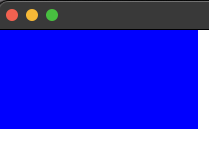
\includegraphics[width=1.0\textwidth]{/Users/ducasse/Workspace/FirstCircle/MyBooks/Bk-Writing/PharoBooks2/Booklet-Graphics/Chapters/bloc/figures/basicElement.png}
\caption{basic element}
\end{center}
\end{figure}


\begin{enumerate}
    \item \textbf{Start with a blank canvas:} Begin by creating a new BlElement. This serves
\end{enumerate}

as the foundation for your user interface element, initially appearing
invisible.

\begin{enumerate}
    \item \textbf{Define its shape:} In Bloc, the element's visual representation is
\end{enumerate}

determined by its geometry. In this example, we'll use a simple rectangle, but
more complex shapes are also possible (explored in further detail later).

\begin{enumerate}
    \item \textbf{Set its dimensions and appearance:} Specify the element's size and color
\end{enumerate}

to customize its visual characteristics.

\begin{enumerate}
    \item \textbf{Bring it to life:} Finally, open the element in a new space, making it
\end{enumerate}

visible on the screen.

\chapter{element shape \& color}
\section{geometry of BlElement}
In Bloc, the visual form and boundaries of your UI elements are determined by
their geometries. Each element can only possess a single geometry, essentially
acting as a blueprint for its shape and size. You can visualize an element as a
specific geometry encapsulated within an invisible rectangular container,
representing its overall \textit{bounds}.

Bloc provides a diverse range of pre-defined geometry shapes accessible through\textcode{BlElementGeometry allSubclasses}. This comprehensive library empowers you to
construct elements of varying complexities, from basic rectangles and circles to
more intricate forms.

Bloc excels in facilitating the creation of custom components with advanced
layout possibilities. Imagine building complex layouts by strategically
arranging various elements, each defined by its unique geometry, to form a
cohesive whole.

While Alexandrie canvas provides a foundational set of building drawing
primitives, Bloc offers a richer library of pre-defined shapes and the
flexibility to construct even more intricate geometries.

\begin{figure}[htpb]
\begin{center}
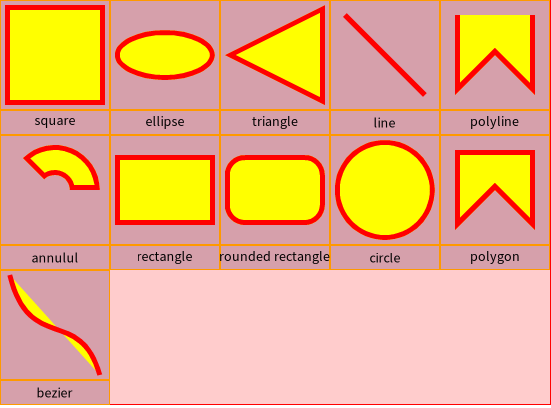
\includegraphics[width=1.0\textwidth]{/Users/ducasse/Workspace/FirstCircle/MyBooks/Bk-Writing/PharoBooks2/Booklet-Graphics/Chapters/bloc/figures/allGeometry.png}
\caption{base geometry}
\end{center}
\end{figure}


\begin{itemize}
    \item \textbf{Annulus} : \textcode{BlAnnulusSectorGeometry new startAngle: 225; endAngle: 360;   innerRadius: 0.3; outerRadius: 0.9);}
    \item \textbf{bezier} : \textcode{BlBezierCurveGeometry controlPoints: \{ 5@0. 25@80. 75@30. 95@100 \}}
    \item \textbf{circle} : \textcode{BlCircleGeometry new matchExtent: 100 @ 50}
    \item \textbf{ellipse} : \textcode{BlEllipseGeometry new matchExtent: 100 @ 50)}
    \item \textbf{line} : \textcode{BlLineGeometry from: 10@10 to: 90@90}
    \item \textbf{Polygon} : \textcode{BlPolygonGeometry vertices: \{(10 @ 10). (10 @ 90). (50 @ 50). (90 @ 90). (90 @ 10)\}}
    \item \textbf{Polyline}: \textcode{BlPolylineGeometry vertices: \{(10 @ 10). (10 @ 90). (50 @ 50).(90 @ 90). (90 @ 10) \}}
    \item \textbf{Rectangle} : \textcode{BlRectangleGeometry  new}
    \item \textbf{Rounded rectangle} : \textcode{BlRoundedRectangleGeometry cornerRadius: 20}
    \item \textbf{square} : \textcode{BlSquareGeometry new matchExtent: 70 @ 70}
    \item \textbf{triangle} : \textcode{BlTriangleGeometry new matchExtent: 50 @ 100; beLeft}
\end{itemize}

\section{element border}
The geometry is like a an invisible line on which your border is painted. The
painting is a subclass of \textbf{BlPaint}, and one of the three:

\begin{itemize}
    \item solid color
    \item linear gradient color
    \item radial gradient color
\end{itemize}

\begin{figure}[htpb]
\begin{center}
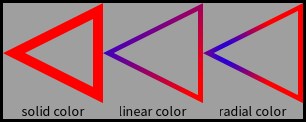
\includegraphics[width=1.0\textwidth]{/Users/ducasse/Workspace/FirstCircle/MyBooks/Bk-Writing/PharoBooks2/Booklet-Graphics/Chapters/bloc/figures/bordercolortype.png}
\caption{border color type}
\end{center}
\end{figure}


Your border opacity can be specified as well: \textcode{opacity: 0.5;}

By default, your border will be a full line, but it can also be dashed, with\textbf{dash array} and \textbf{dash offset}. Dash array define the number of element, and
dash offset, the space between elements.

You also have pre-defined option, available in a single call:

\begin{itemize}
    \item \textbf{dashed}
    \item \textbf{dashed small}
\end{itemize}

\begin{figure}[htpb]
\begin{center}
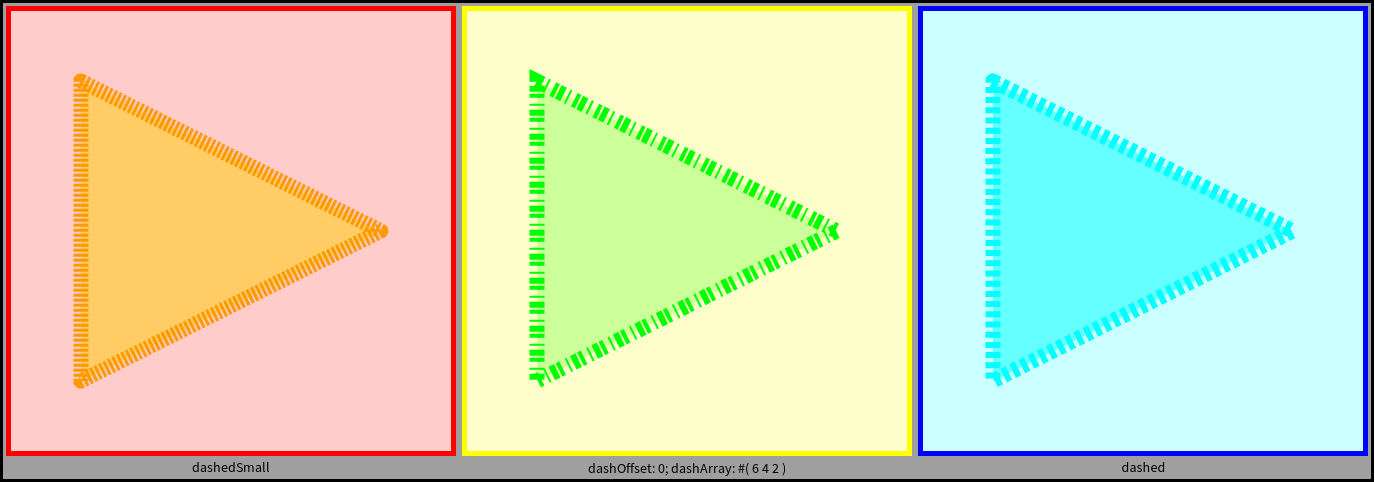
\includegraphics[width=1.0\textwidth]{/Users/ducasse/Workspace/FirstCircle/MyBooks/Bk-Writing/PharoBooks2/Booklet-Graphics/Chapters/bloc/figures/multipletriangledash.png}
\caption{border dash}
\end{center}
\end{figure}


If the path is not closed, The style extent of your border can be defined with

\begin{itemize}
    \item \textbf{cap square}
    \item \textbf{cap round}
    \item \textbf{cap butt}
\end{itemize}

Last, when the line of your border cross each other, you can define the style of
the join:

\begin{itemize}
    \item \textbf{round join}
    \item \textbf{bevel join}
    \item \textbf{mitter join}
\end{itemize}

\begin{figure}[htpb]
\begin{center}
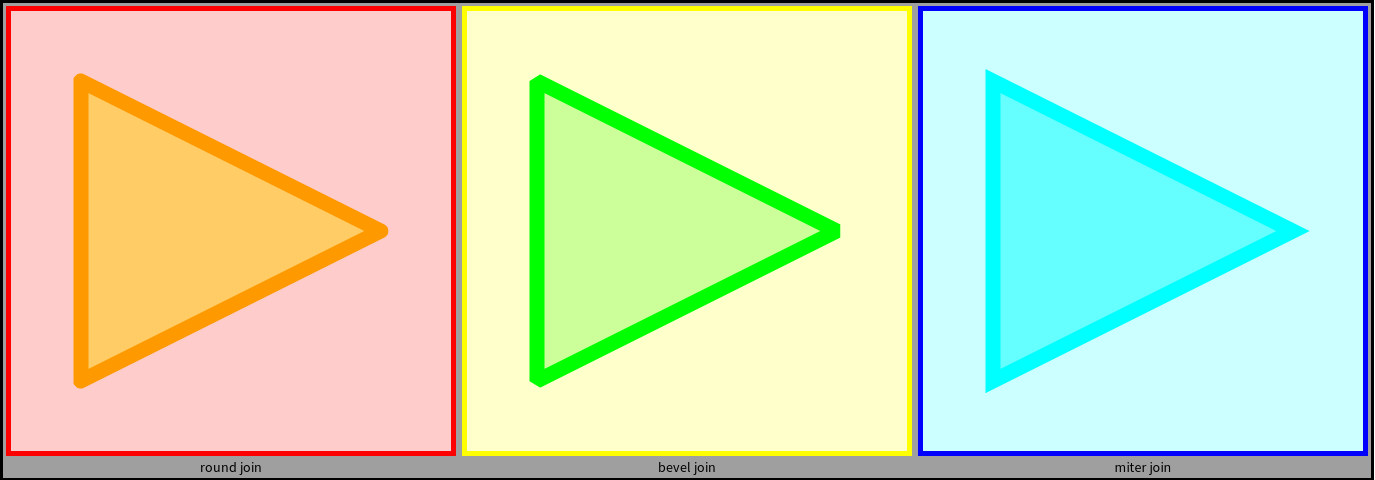
\includegraphics[width=1.0\textwidth]{/Users/ducasse/Workspace/FirstCircle/MyBooks/Bk-Writing/PharoBooks2/Booklet-Graphics/Chapters/bloc/figures/borderjointype.png}
\caption{border join type}
\end{center}
\end{figure}


You have two option to define your border:

\begin{itemize}
    \item short call : \textcode{border: (BlBorder paint: Color orange width: 5)}
    \item with a builder :\textcode{BlBorder builder dashed; paint: Color red; width: 3; build}
\end{itemize}

The first one is very helpfull for solid line definition. The builder let use
customize all the detail of your border.

\section{elements bounds and outskirts}
Lets look at the diffent possible bounds of your element.

\textbf{Layout bounds} can be defined explicitly using \textbf{size:} method or dynamicaly
Layout bounds are considered by layout algorithms to define mutual locations
for all considered elements. You'll know more about layout later.

\textbf{Geometry bounds} area is defined by minimum and maximum values of polygon
vertices. This does not take in account the border width

\textbf{Visual bounds} is an exact area occupied by an element. it takes strokes
and rendering into account.

The geometry is like a an invisible line on which your border is represented.
The border drawing can happen outside (adding its border size to the size of
your element), centered, or inside the geometry of the element. The final size
(geometry + border width) will define the \textbf{bounds} of your element.

In this figure, the same exact star is drawned 3 time. The only difference is
the outskirts definition between those 3.

\begin{figure}[htpb]
\begin{center}
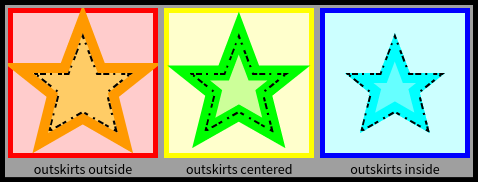
\includegraphics[width=1.0\textwidth]{/Users/ducasse/Workspace/FirstCircle/MyBooks/Bk-Writing/PharoBooks2/Booklet-Graphics/Chapters/bloc/figures/multipletriangleoutskirts.png}
\caption{outskirts}
\end{center}
\end{figure}


If we specify BlOutskirts inside, visual bound and geometry bounds will be the
same. But if BlOutskirts is outside, then visual bounds are larger than
geometry bounds to take border width into its calculation.

\section{element background}
quick set-up: \textcode{background: (Color red alpha: 0.8);}

using rgb color
\begin{displaycode}{smalltalk}
background: (Color r: 63 g: 81           b: 181     range: 255);
\end{displaycode}

using linear gradient
\begin{displaycode}{smalltalk}
background: ((BlLinearGradientPaint direction: 1 @ 1) from: Color red to: Color blue).
\end{displaycode}

using radial gradient
\begin{displaycode}{smalltalk}
background: (BlRadialGradientPaint new
stops: { 0 -> Color blue. 1 -> Color red };
center: largeExtent // 2;
radius: largeExtent min;
yourself);
\end{displaycode}

Using dedicated \textit{BlPaintBackground} object.
\begin{displaycode}{smalltalk}
background: ((BlPaintBackground paint: fillColor asBlPaint) opacity: 0.75; yourself);
\end{displaycode}

\begin{figure}[htpb]
\begin{center}
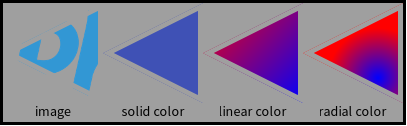
\includegraphics[width=1.0\textwidth]{/Users/ducasse/Workspace/FirstCircle/MyBooks/Bk-Writing/PharoBooks2/Booklet-Graphics/Chapters/bloc/figures/backgroundcolortype.png}
\caption{background color}
\end{center}
\end{figure}


\section{element effect}
\textcode{BlElementEffect allSubclasses}
\begin{displaycode}{smalltalk}
BlElement new
        size: 200 @ 100;
        geometry: (BlRoundedRectangleGeometry cornerRadius: 2);
        background: (Color red alpha: 0.2);
        border: (BlBorder paint: Color yellow width: 1);
        outskirts: BlOutskirts centered;
        effect:
            (BlSimpleShadowEffect color: Color orange offset: -10 @ -20)
\end{displaycode}

\begin{figure}[htpb]
\begin{center}

\includegraphics[width=1.0\textwidth]{/Users/ducasse/Workspace/FirstCircle/MyBooks/Bk-Writing/PharoBooks2/Booklet-Graphics/Chapters/bloc/figures/simpleshadow.png}
\caption{simple shadow}
\end{center}
\end{figure}


effect: (BlSimpleShadowEffect
color: (Color orange alpha: shadowAlpha)
offset: shadowOffset);
\begin{displaycode}{smalltalk}
BlElement new
        size: 300 @ 150;
        geometry: (BlRoundedRectangleGeometry cornerRadius: 2);
        background: (Color blue alpha: 0.5);
        border: (BlBorder paint: Color red width: 10);
        effect: (BlGaussianShadowEffect color: Color yellow offset: 10@20 width: 5)
\end{displaycode}

\begin{figure}[htpb]
\begin{center}
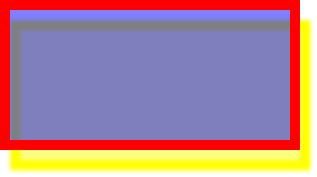
\includegraphics[width=1.0\textwidth]{/Users/ducasse/Workspace/FirstCircle/MyBooks/Bk-Writing/PharoBooks2/Booklet-Graphics/Chapters/bloc/figures/gaussianshadow.png}
\caption{gaussian shadow}
\end{center}
\end{figure}


\section{element opacity}
\textcode{element opacity:}, value between 0 and 1, 0 meaning completely transparent
You can apply opacity to background, border, or to your hole element.

\begin{figure}[htpb]
\begin{center}
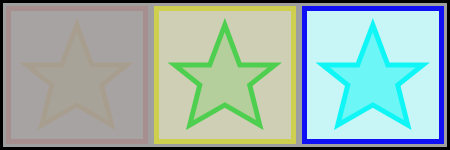
\includegraphics[width=1.0\textwidth]{/Users/ducasse/Workspace/FirstCircle/MyBooks/Bk-Writing/PharoBooks2/Booklet-Graphics/Chapters/bloc/figures/elementwitopacity.png}
\caption{element opacity}
\end{center}
\end{figure}


\chapter{element transformation}
You can apply transformation to a BlElement:

\begin{itemize}
    \item rotation
    \item translation
    \item Scaling
    \item reflection
    \item etc...
\end{itemize}

transformDo: {[} :b \textbar{} b scaleBy: 0.2; translateBy: -25 @ -15 {]};
\begin{displaycode}{smalltalk}
aContainer := BlElement new
                    layout: BlFrameLayout new;
                    constraintsDo: [ :c |
                        c horizontal fitContent.
                        c vertical fitContent ];
                    padding: (BlInsets all: 20);
                    background: (Color gray alpha: 0.2).

node := BlElement new
            geometry: (BlRoundedRectangleGeometry cornerRadius: 4);
            border: (BlBorder paint: Color black width: 2);
            background: Color white;
            constraintsDo: [ :c |
                c frame horizontal alignCenter.
                c frame vertical alignBottom ];
            size: 20 @ 20.

aContainer transformDo: [ :t |
    t
        scaleBy: 2.0;
        rotateBy: 69;
        translateBy: 50 @ 50 ].
aContainer addChild: node.

aContainer forceLayout.
\end{displaycode}

\begin{figure}[htpb]
\begin{center}
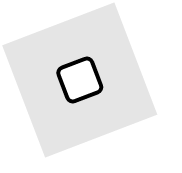
\includegraphics[width=1.0\textwidth]{/Users/ducasse/Workspace/FirstCircle/MyBooks/Bk-Writing/PharoBooks2/Booklet-Graphics/Chapters/bloc/figures/transformexample.png}
\caption{transform example}
\end{center}
\end{figure}


A few hint on using transormDo:

\begin{itemize}
    \item transformDo: can be applied at any moment during the life of an object.
    \item you can use any static or pre-compute properties with transformDo:
    \item if you want to use dynamic layout properties (like size) with \textit{transformDo}:, you need to wait for layout phase to be completed.
\end{itemize}

\chapter{Bloc styles}
\chapter{element custom Painting}
Bloc really favor BlElement composition to create your interface. Most of the
time, you will not have to create a custom painting of your element widget. You
can already do a lot with existing geometry.

Ultimately, you can define
drawing methods on a canvas, but once drawn, a canvas cannot be easily inspected
for its elements. However, Bloc element composition create a tree of elements,
that can be inspected, and shaped dynamically.

creating and drawing your own block
=\textgreater{} subclass BlElement
=\textgreater{} Custom drawing is done with drawOnSpartaCanvas: method.
=\textgreater{}

BlElement \textgreater{}\textgreater{} aeFullDrawOn: aCanvas
\symbol{34}Main entry point to draw myself and my children on an Alexandrie canvas.\symbol{34}

self aeDrawInSameLayerOn: aCanvas.

self aeCompositionLayersSortedByElevationDo: {[} :each \textbar{} each paintOn: aCanvas {]}.

Element geometry is taken care by:
BlElement \textgreater{}\textgreater{} aeDrawGeometryOn: aeCanvas
Painting is done on an Alexandrie Canvas, then rendered on the host:
BARenderer (BlHostRenderer) \textgreater{}\textgreater{} render: aHostSpace, display on a AeCairoImageSurface

Drawing is done through method 'drawOnSpartaCanvas', which receive a sparta
(vector) canvas as an argument.

\begin{enumerate}
    \item aeDrawChildrenOn:
    \item aeDrawOn:
    \item aeDrawGeometryOn:
\end{enumerate}

\chapter{UI Building}
\textless{}\href{https://github.com/OpenSmock/Pyramid/tree/main>}{https://github.com/OpenSmock/Pyramid/tree/main\textgreater{}}



\bibliographystyle{alpha}
\bibliography{book.bib}

% lulu requires an empty page at the end. That's why I'm using
% \backmatter here.
\backmatter

% Index would go here

\end{document}
